\documentclass[aspectratio=169]{beamer}

% Pacotes essenciais
\usepackage[utf8]{inputenc}
\usepackage[T1]{fontenc}
\usepackage[brazilian]{babel}
\usepackage{graphicx}
\usepackage{tikz}

% Fonte moderna Roboto
\usepackage[sfdefault]{roboto}
\usepackage[T1]{fontenc}

% Definição das cores
\definecolor{vermelhoPrincipal}{HTML}{b11116}
\definecolor{azulComplementar}{HTML}{3a5461}
\definecolor{brancoFundo}{HTML}{FFFFFF}

% Configuração do tema
\usetheme{Madrid}
\usecolortheme{default}

% Cores personalizadas - texto sempre em preto
\setbeamercolor{structure}{fg=black}
\setbeamercolor{palette primary}{bg=vermelhoPrincipal,fg=white}
\setbeamercolor{palette secondary}{bg=azulComplementar,fg=white}
\setbeamercolor{palette tertiary}{bg=vermelhoPrincipal,fg=white}
\setbeamercolor{palette quaternary}{bg=azulComplementar,fg=white}
\setbeamercolor{frametitle}{bg=vermelhoPrincipal,fg=white}
\setbeamercolor{background canvas}{bg=brancoFundo}
\setbeamercolor{title}{fg=black}
\setbeamercolor{subtitle}{fg=azulComplementar}
\setbeamercolor{author}{fg=black}
\setbeamercolor{date}{fg=black}
\setbeamercolor{itemize item}{fg=black}
\setbeamercolor{itemize subitem}{fg=black}
\setbeamercolor{enumerate item}{fg=black}
\setbeamercolor{block title}{bg=vermelhoPrincipal,fg=white}
\setbeamercolor{block body}{bg=vermelhoPrincipal!10,fg=black}
\setbeamercolor{normal text}{fg=black}

% Configurar fonte dos itemize
\setbeamerfont{itemize/enumerate body}{size=\scriptsize}
\setbeamerfont{itemize/enumerate subbody}{size=\scriptsize}

% Marcadores modernos e minimalistas
\setbeamertemplate{itemize item}{\raisebox{0.2ex}{\rule{0.6ex}{0.6ex}}}
\setbeamertemplate{itemize subitem}{\raisebox{0.3ex}{\rule{0.4ex}{0.4ex}}}
\setbeamertemplate{itemize subsubitem}{\raisebox{0.35ex}{\rule{0.3ex}{0.3ex}}}
\setbeamertemplate{enumerate items}[square]

% Transições suaves
\setbeamercovered{transparent}

% Remover símbolos de navegação
\setbeamertemplate{navigation symbols}{}

% Customizar o cabeçalho com barra vermelha e logo
\setbeamertemplate{headline}{
  \begin{beamercolorbox}[wd=\paperwidth,ht=0.6cm,dp=0.15cm,leftskip=0.2cm,rightskip=0.4cm]{palette primary}
    \raisebox{-0.05cm}{
\includegraphics[height=0.45cm]{imgs/base/fatec-rgt.png}}
    \hfill
    \raisebox{-0.18cm}{
\includegraphics[height=0.85cm]{imgs/base/governo-sp-secretaria-logo.png}}
    \hspace{0.2cm}
    \raisebox{-0.08cm}{
\includegraphics[height=0.6cm]{imgs/base/cps-logo.png}}
  \end{beamercolorbox}
}
% Remover sombras dos blocks
\setbeamertemplate{blocks}[default]
\setbeamertemplate{itemize/enumerate body begin}{\scriptsize}
\setbeamertemplate{itemize/enumerate subbody begin}{\scriptsize}
% Customizar o rodapé
\setbeamertemplate{footline}{
  \begin{beamercolorbox}[wd=\paperwidth,ht=0.4cm,dp=0.2cm,leftskip=0.3cm,rightskip=0.3cm]{palette secondary}
    \usebeamerfont{footline}
    \insertshortauthor \hfill \hfill {\fontsize{5}{6}\selectfont\insertshorttitle} \hfill \hfill \insertframenumber/\inserttotalframenumber
  \end{beamercolorbox}
}

% Customizar título do frame
\setbeamertemplate{frametitle}{
  \vspace{0.3cm}
  \textcolor{black}{\insertframetitle}
  \vspace{0.1cm}
}

% Informações da apresentação
\title{Classificação de Manganês na Folha da Mexerica, \\ Orientado por Redes Neurais}
\subtitle{}
\author[DSM]{ALVES, A; FAGUNDES, L.; FREITAS, V.; RODRIGUES, J.}
\institute{Desenvolvimento de Software Multiplataforma\\FATEC Registro}
\date{\today}

\begin{document}

% Slide de título moderno
\begin{frame}
  \vspace{0.8cm}
  \begin{center}
    \begin{tikzpicture}
      % Linha decorativa superior
      \draw[vermelhoPrincipal, line width=2pt] (-4,0) -- (4,0);
    \end{tikzpicture}
    
    \vspace{0.4cm}
    
    {\normalsize\bfseries\inserttitle}\par
    
    \vspace{0.2cm}
    
    {\tiny\insertauthor}\par
    
    \vspace{0.1cm}
    
    {\small\textcolor{azulComplementar}{\insertsubtitle}}\par
    
    \vspace{0.5cm}
    
    \begin{tikzpicture}
      % Linha decorativa inferior
      \draw[azulComplementar, line width=1.5pt] (-2.5,0) -- (2.5,0);
    \end{tikzpicture}
    
    \vspace{0.3cm}
    
    {\scriptsize\insertinstitute}\par
    
    \vspace{0.01cm}
    
    {\tiny\textcolor{azulComplementar}{\insertdate}}\par
  \end{center}
\end{frame}

% Slide de agenda
\begin{frame}[b]{Agenda}
  \begin{itemize}
    \item Pitch
    \item Problematização
    \item Objetivo
    \item Estado da Arte
    \item Ferramental
    \item Metodologia
    \item Apresentação prática
    \item Resultados e Discussões
  \end{itemize}
  
  \vfill
  
  \hfill{\scriptsize \textbf{Duração:} 10 a 11 min.}
\end{frame}

\section{Pitch}
{
\usebackgroundtemplate{%
  
\includegraphics[width=\paperwidth,height=\paperheight]{imgs/Pitch.png}%
}
\begin{frame}[b]{Pitch}
  \begin{itemize}
    \item \parbox{0.60\textwidth}{Apresentação concisa e objetiva do projeto}
    \item \parbox{0.60\textwidth}{Destaque do \textbf{problema} que o projeto resolve}
    \item \parbox{0.60\textwidth}{Proposta de \textbf{valor} e diferenciais da solução}
    \item \parbox{0.60\textwidth}{Público-alvo e \textbf{impacto} esperado}
    \item \parbox{0.60\textwidth}{Visão geral das \textbf{tecnologias} utilizadas}
  \end{itemize}
  
  \vfill
  
  {\fontsize{4}{5}\selectfont\textit{Fonte: Seu Nome}\hfill\textcolor{white}{Imagem: Descrição da imagem}}
\end{frame}
}

\section{Problematização}

{
\usebackgroundtemplate{%
  
\includegraphics[width=\paperwidth,height=\paperheight]{imgs/img_002.jpg}%
}
\begin{frame}[b]{Problematização}
  \begin{itemize}
    \item \parbox{0.60\textwidth}{Contextualização do \textbf{problema} identificado}
    \item \parbox{0.60\textwidth}{Análise das \textbf{causas} e consequências}
    \item \parbox{0.60\textwidth}{Impacto no público-alvo ou na área de atuação}
    \item \parbox{0.60\textwidth}{Justificativa da \textbf{relevância} do projeto}
    \item \parbox{0.60\textwidth}{Lacunas nas soluções existentes}
  \end{itemize}
  
  \vfill
  
  {\fontsize{4}{5}\selectfont\textit{Fonte: Seu Nome}\hfill\textcolor{white}{Imagem: Descrição da imagem}}
\end{frame}
}

\section{Objetivo}

{
\usebackgroundtemplate{%
  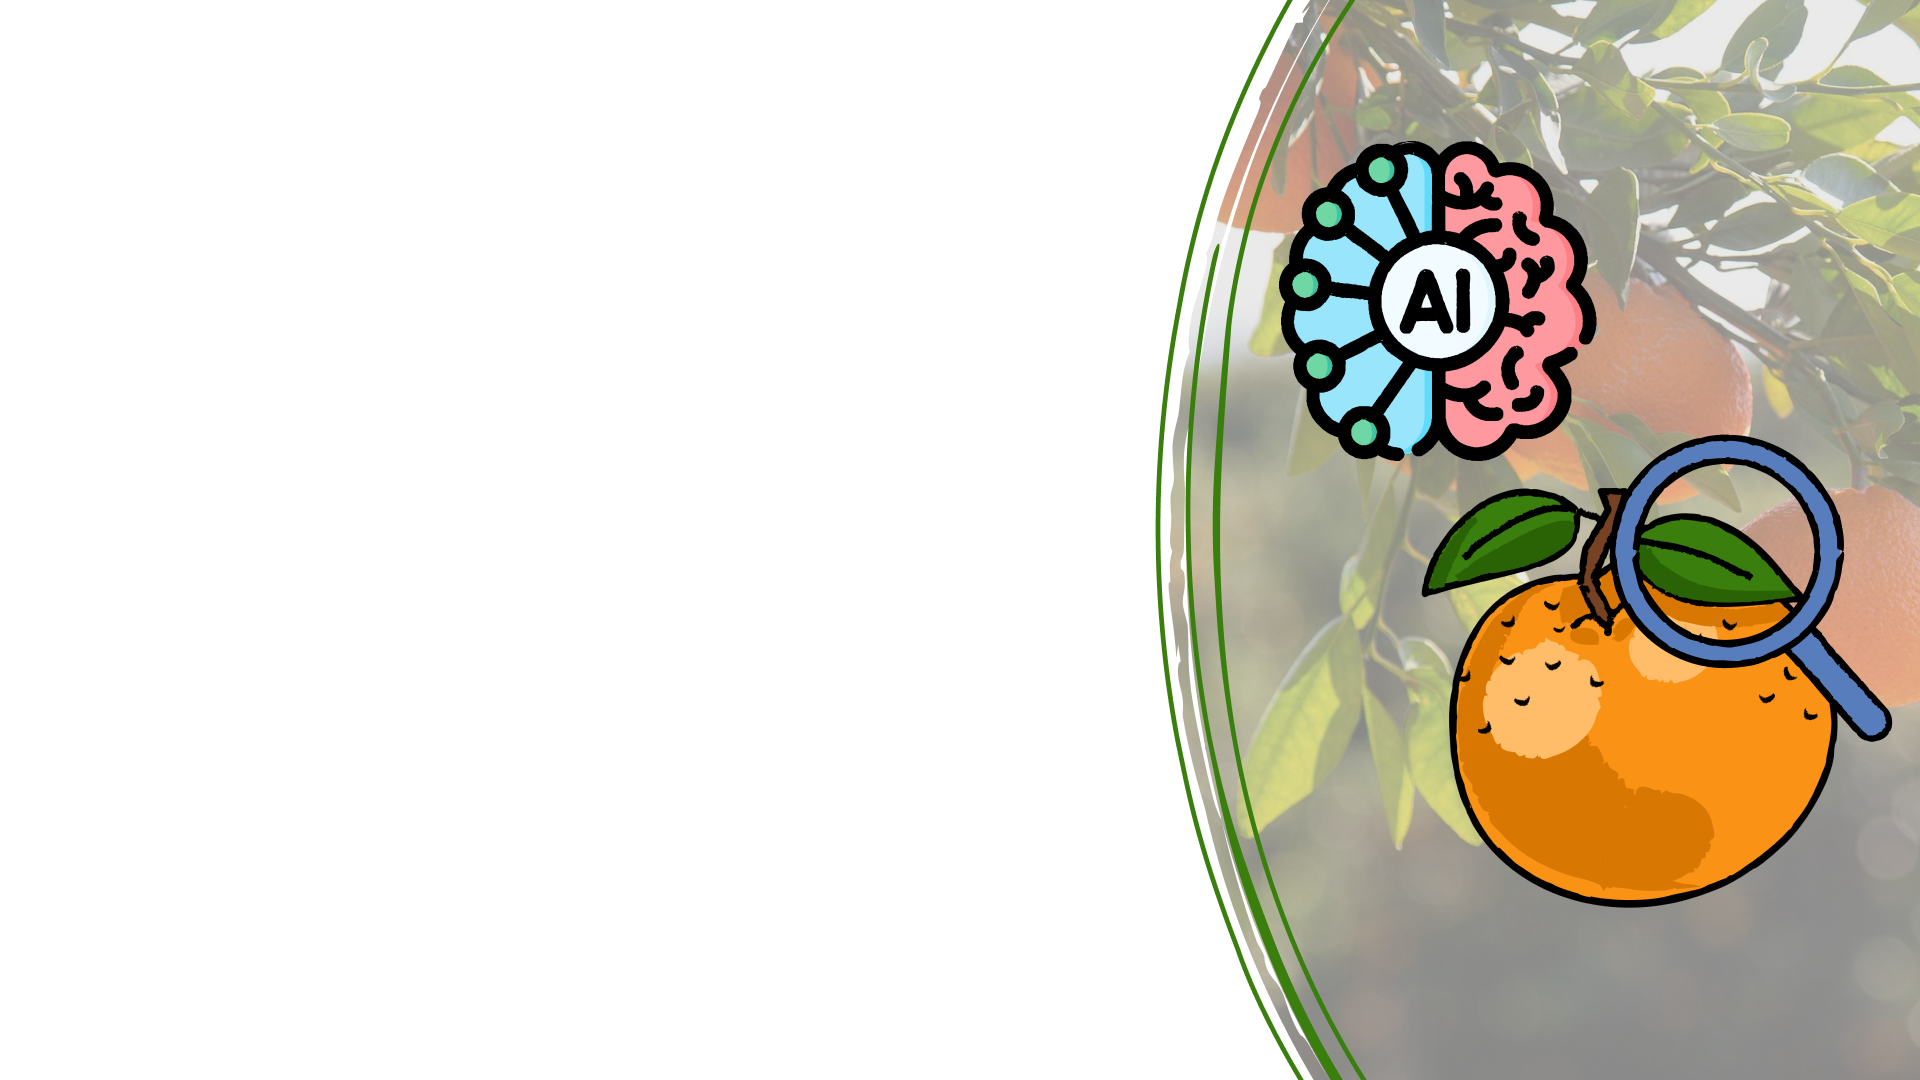
\includegraphics[width=\paperwidth,height=\paperheight]{imgs/Objetivos.png}%
}
\begin{frame}[b]{Objetivo}
  \begin{itemize}
    \item \parbox{0.60\textwidth}{\textbf{Objetivo geral}: Desenvolver o \textbf{NitrusLeaf}, para identificar \\deficiência nutricional em folhas de mexerica com IA.}
    \vspace{0.3cm}
    \item \parbox{0.60\textwidth}{\textbf{Objetivos específicos}:}
    
    \begin{itemize}
      \item \parbox{0.55\textwidth}{Criar banco de imagens rotuladas.}
      \item \parbox{0.55\textwidth}{Treinar e validar a CNN.}
      \item \parbox{0.55\textwidth}{Desenvolver aplicativo móvel}
    \end{itemize}
    \vspace{0.3cm}
    \item \parbox{0.60\textwidth}{Resultados esperados e \textbf{entregas}: Aplicativo funcional e acessível,\\ com modelo de IA validado e base de dados organizada.}
    \vspace{0.3cm}
    \item \parbox{0.60\textwidth}{Métricas de \textbf{sucesso}: Alta acurácia, diagnóstico mais rápido,\\ facilidade de uso e possibilidade de expansão futura.}
  \end{itemize}
  
  \vfill
  
  {\fontsize{4}{5}\selectfont\textit{Fonte: Seu Nome}\hfill\textcolor{white}{Imagem: Descrição da imagem}}
\end{frame}
}

% ESTADO DA ARTE --------------------------------------------------------------------------------
\section{Estado da Arte}

% ESTADO DA ARTE 1
\begin{frame}[t]{Estado da Arte}
  \scriptsize
  
  Abordagens Baseadas em Visão Computacional, Aprendizado de
  Máquina e Aprendizado Profundo para Identificação de Deficiências
  Nutricionais em Culturas
  
  \vspace{0.3cm}
  
  \begin{table}
    \centering
    \tiny
    \begin{tabular}{|p{2.5cm}|p{2cm}|p{2cm}|p{2cm}|p{2cm}|p{1.5cm}|}
      \hline
      \textbf{Título/Autores} & \textbf{Objetivo} & \textbf{Método} & \textbf{Resultados} & \textbf{Limitações} & \textbf{Gap} \\
      \hline
      Computer Vision Based Machine Learning and Deep Learning Approaches for Identification of Nutrient Deficiency in Crops: A Survey - Sudhakar e Swarna Priya (2023)
      & Revisar técnicas de visão computacional para detectar deficiência nutricional em plantas
      & Survey de trabalhos com ML, DL, UAVs, IoT e sensoriamento remoto
      & CNNs, UAVs e IoT apresentaram bons resultados na identificação de deficiências
      & Dependência de grandes bases de dados e dificuldade em diferentes ambientes
      & Falta de sistemas em tempo real e foco limitado em micronutrientes
      \\
      \hline

    \end{tabular}
  \end{table}
\end{frame}

% ESTADO DA ARTE 2
\begin{frame}[t]{Estado da Arte}
  \scriptsize

  Detecção de Doenças e Deficiências Nutricionais em Plantas
  Baseada em Processamento de Imagens

  \vspace{0.3cm}
  
  \begin{table}
    \centering
    \tiny
    \begin{tabular}{|p{2.5cm}|p{2cm}|p{2cm}|p{2cm}|p{2cm}|p{1.5cm}|}
      \hline
      \textbf{Título/Autores} & \textbf{Objetivo} & \textbf{Método} & \textbf{Resultados} & \textbf{Limitações} & \textbf{Gap} \\
      \hline
      Image Processing Based Detection of Diseases and Nutrient Deficiencies in Plants - Ghorai et al. (2021)
      & Revisar técnicas de processamento de imagens para detectar doenças e deficiências nutricionais em plantas
      & Survey sobre visão computacional, segmentação, extração de características e classificadores de ML
      & CNNs, SVM e imagens hiperespectrais apresentaram alta eficiência na detecção de doenças e deficiências
      & Sensível a iluminação, ruídos e variações ambientais durante captura das imagens
      & Necessidade de sistemas mais robustos, automáticos e em tempo real para uso em campo
      \\
      \hline

    \end{tabular}
  \end{table}
\end{frame}

% ESTADO DA ARTE 3
\begin{frame}[t]{Estado da Arte}
  \scriptsize
  
  Um Estudo Comparativo de Deep CNN Na Previsão e Classificação
  de Deficiências de Macronutrientes no Desenvolvimento de Plantas
  de Tomate
  \vspace{0.3cm}
  
  \begin{table}
    \centering
    \tiny
    \begin{tabular}{|p{2.5cm}|p{2cm}|p{2cm}|p{2cm}|p{2cm}|p{1.5cm}|}
      \hline
      \textbf{Título/Autores} & \textbf{Objetivo} & \textbf{Método} & \textbf{Resultados} & \textbf{Limitações} & \textbf{Gap} \\
      \hline
      A Comparative Study of Deep CNN in Forecasting and Classifying the Macronutrient Deficiencies on Development of Tomato Plant - Tran et al. (2019)
      & Classificar e prever deficiências nutricionais em tomateiros utilizando Deep Learning
      & Uso de CNNs (Inception-ResNet v2 e Autoencoder) com imagens de folhas e frutos; aplicação de Ensemble Averaging
      & Acurácia de 87,27\% com Inception-ResNet v2 e 91\% utilizando ensemble learning
      & Dataset reduzido (571 imagens), foco apenas em tomateiros e condições controladas de estufa
      & Necessidade de validação em ambientes reais e adaptação para diferentes culturas agrícolas e micronutrientes
      \\
      \hline

    \end{tabular}
  \end{table}
\end{frame}

\section{Ferramental}

{
\usebackgroundtemplate{%
  
\includegraphics[width=\paperwidth,height=\paperheight]{imgs/img_005.jpg}%
}
\begin{frame}[b]{Ferramental}
  \begin{itemize}
      \item \parbox{0.60\textwidth}{
          \textbf{Linguagens}: Python e JavaScript}
      \item \parbox{0.60\textwidth}{
          \textbf{Frameworks e bibliotecas}: TensorFlow, Keras, React, Next.js e Node.js}
      \item \parbox{0.60\textwidth}{
          \textbf{Banco de dados}: MySQL hospedado no Supabase}
      \item \parbox{0.60\textwidth}{
          \textbf{Infraestrutura}: API de comunicação entre aplicativo e servidor}
      \item \parbox{0.60\textwidth}{
          \textbf{Ferramentas}: Figma, Git e VS Code}
      \item \parbox{0.60\textwidth}{
          \textbf{APIs e integrações}: Integração entre aplicativo móvel, API Node.js e modelo de IA}
  \end{itemize}
  
  \vfill
  
  {\fontsize{4}{5}\selectfont\textit{Fonte: Seu Nome}\hfill\textcolor{white}{Imagem: Descrição da imagem}}
\end{frame}
}

\section{Metodologia}

{
\usebackgroundtemplate{%
  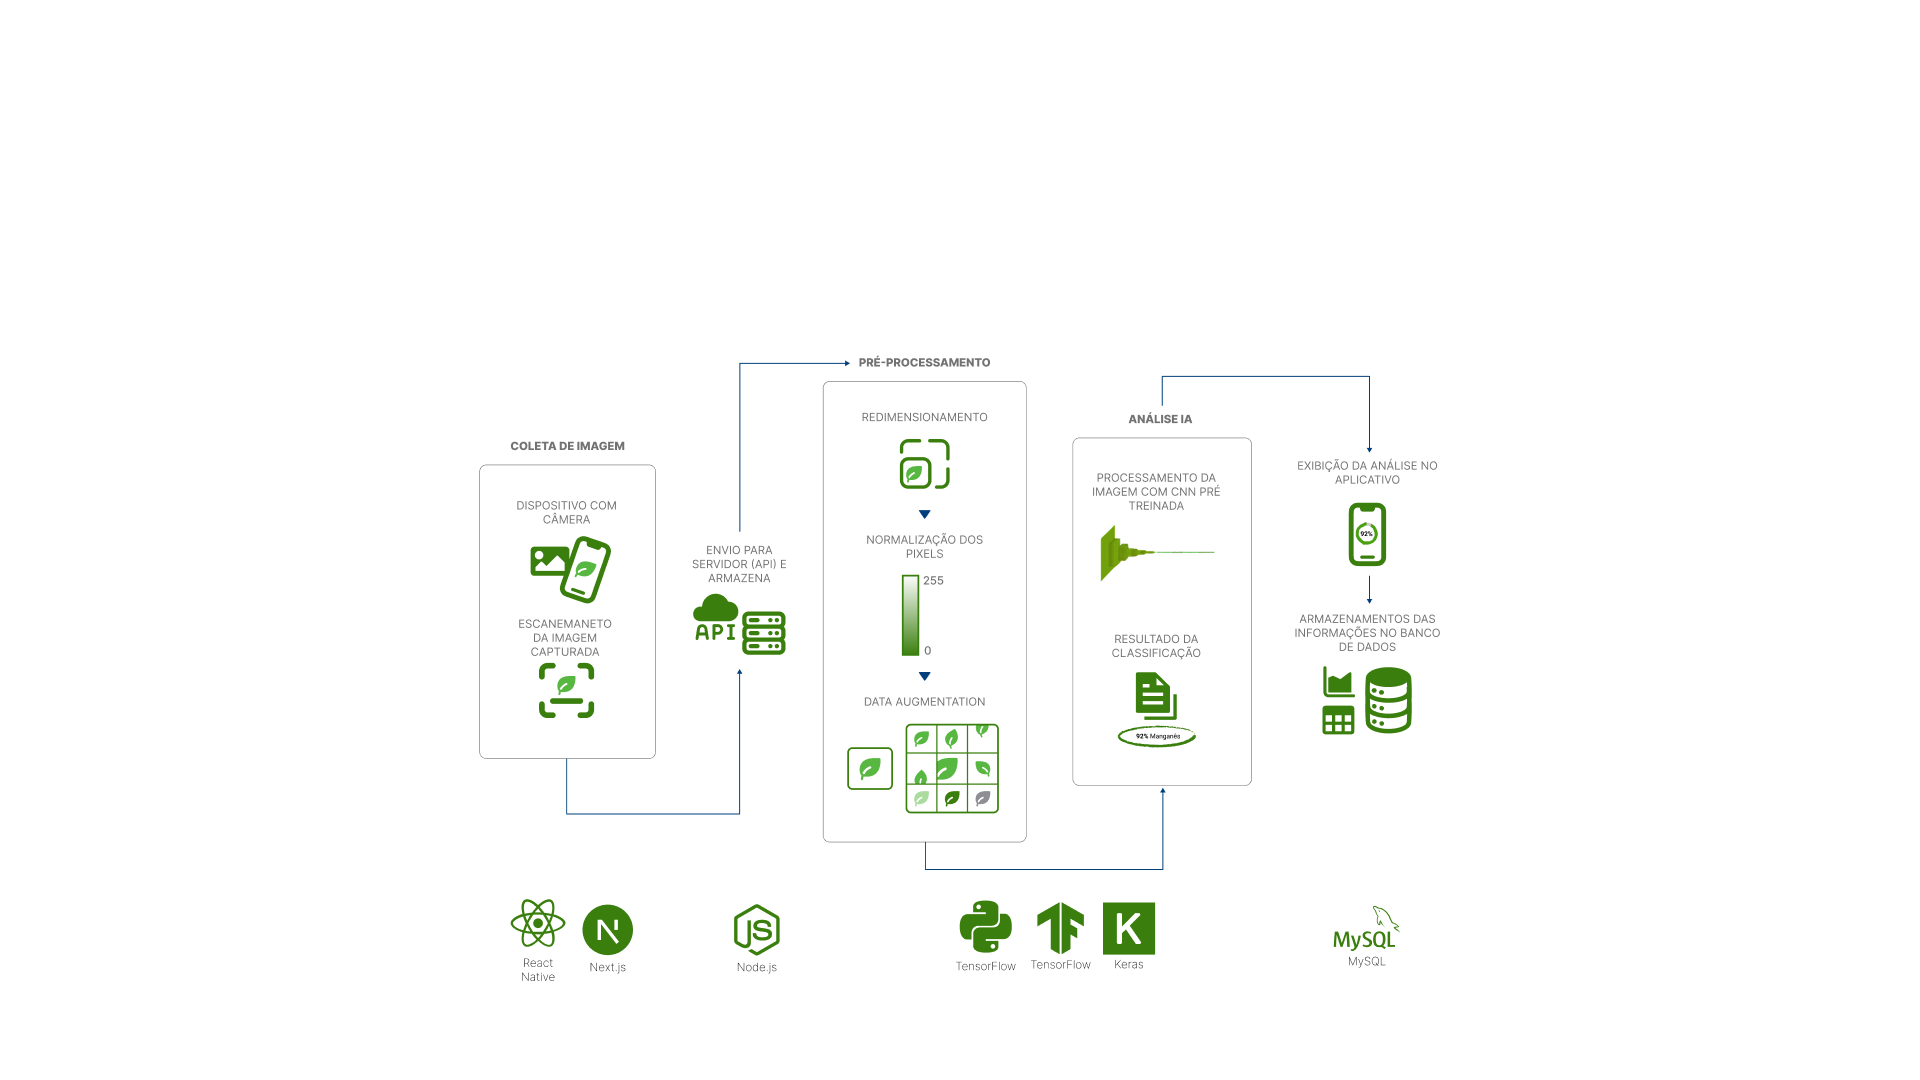
\includegraphics[width=\paperwidth,height=\paperheight]{imgs/Metodologias.png}%
}
\begin{frame}[t]{Metodologia}
  
  \scriptsize
  Fluxograma dos principais processos implementados no projeto, evidenciando as tecnologias empregadas, tais como Inteligência Artificial (IA) e Banco de Dados.

\end{frame}
}

\section{Apresentação Prática}

{
\usebackgroundtemplate{%
  
\includegraphics[width=\paperwidth,height=\paperheight]{imgs/img_007.jpg}%
}
\begin{frame}[b]{Apresentação Prática}
  \begin{itemize}
    \item \parbox{0.60\textwidth}{\textbf{Demonstração} ao vivo do sistema}
    \item \parbox{0.60\textwidth}{Principais \textbf{funcionalidades} implementadas}
    \item \parbox{0.60\textwidth}{\textbf{Interface} e experiência do usuário}
    \item \parbox{0.60\textwidth}{Fluxos de \textbf{uso} e navegação}
    \item \parbox{0.60\textwidth}{Casos de uso e \textbf{cenários} práticos}
  \end{itemize}
  
  \vfill
  
  {\fontsize{4}{5}\selectfont\textit{Fonte: Seu Nome}\hfill\textcolor{white}{Imagem: Descrição da imagem}}
\end{frame}
}

\section{Resultados e Discussões}

{
\usebackgroundtemplate{%
  
\includegraphics[width=\paperwidth,height=\paperheight]{imgs/img_008.jpg}%
}
\begin{frame}[b]{Resultados e Discussões}
  \begin{itemize}
    \item \parbox{0.60\textwidth}{Principais \textbf{resultados} alcançados}
    \item \parbox{0.60\textwidth}{Análise de \textbf{métricas} e indicadores}
    \item \parbox{0.60\textwidth}{Feedback dos \textbf{usuários} e testes realizados}
    \item \parbox{0.60\textwidth}{\textbf{Desafios} encontrados e soluções adotadas}
    \item \parbox{0.60\textwidth}{Contribuições e \textbf{aprendizados} do projeto}
    \item \parbox{0.60\textwidth}{\textbf{Trabalhos futuros} e melhorias propostas}
  \end{itemize}
  
  \vfill
  
  {\fontsize{4}{5}\selectfont\textit{Fonte: Seu Nome}\hfill\textcolor{white}{Imagem: Descrição da imagem}}
\end{frame}
}

% Slide Informações Gerais (clone)
{
\usebackgroundtemplate{%
  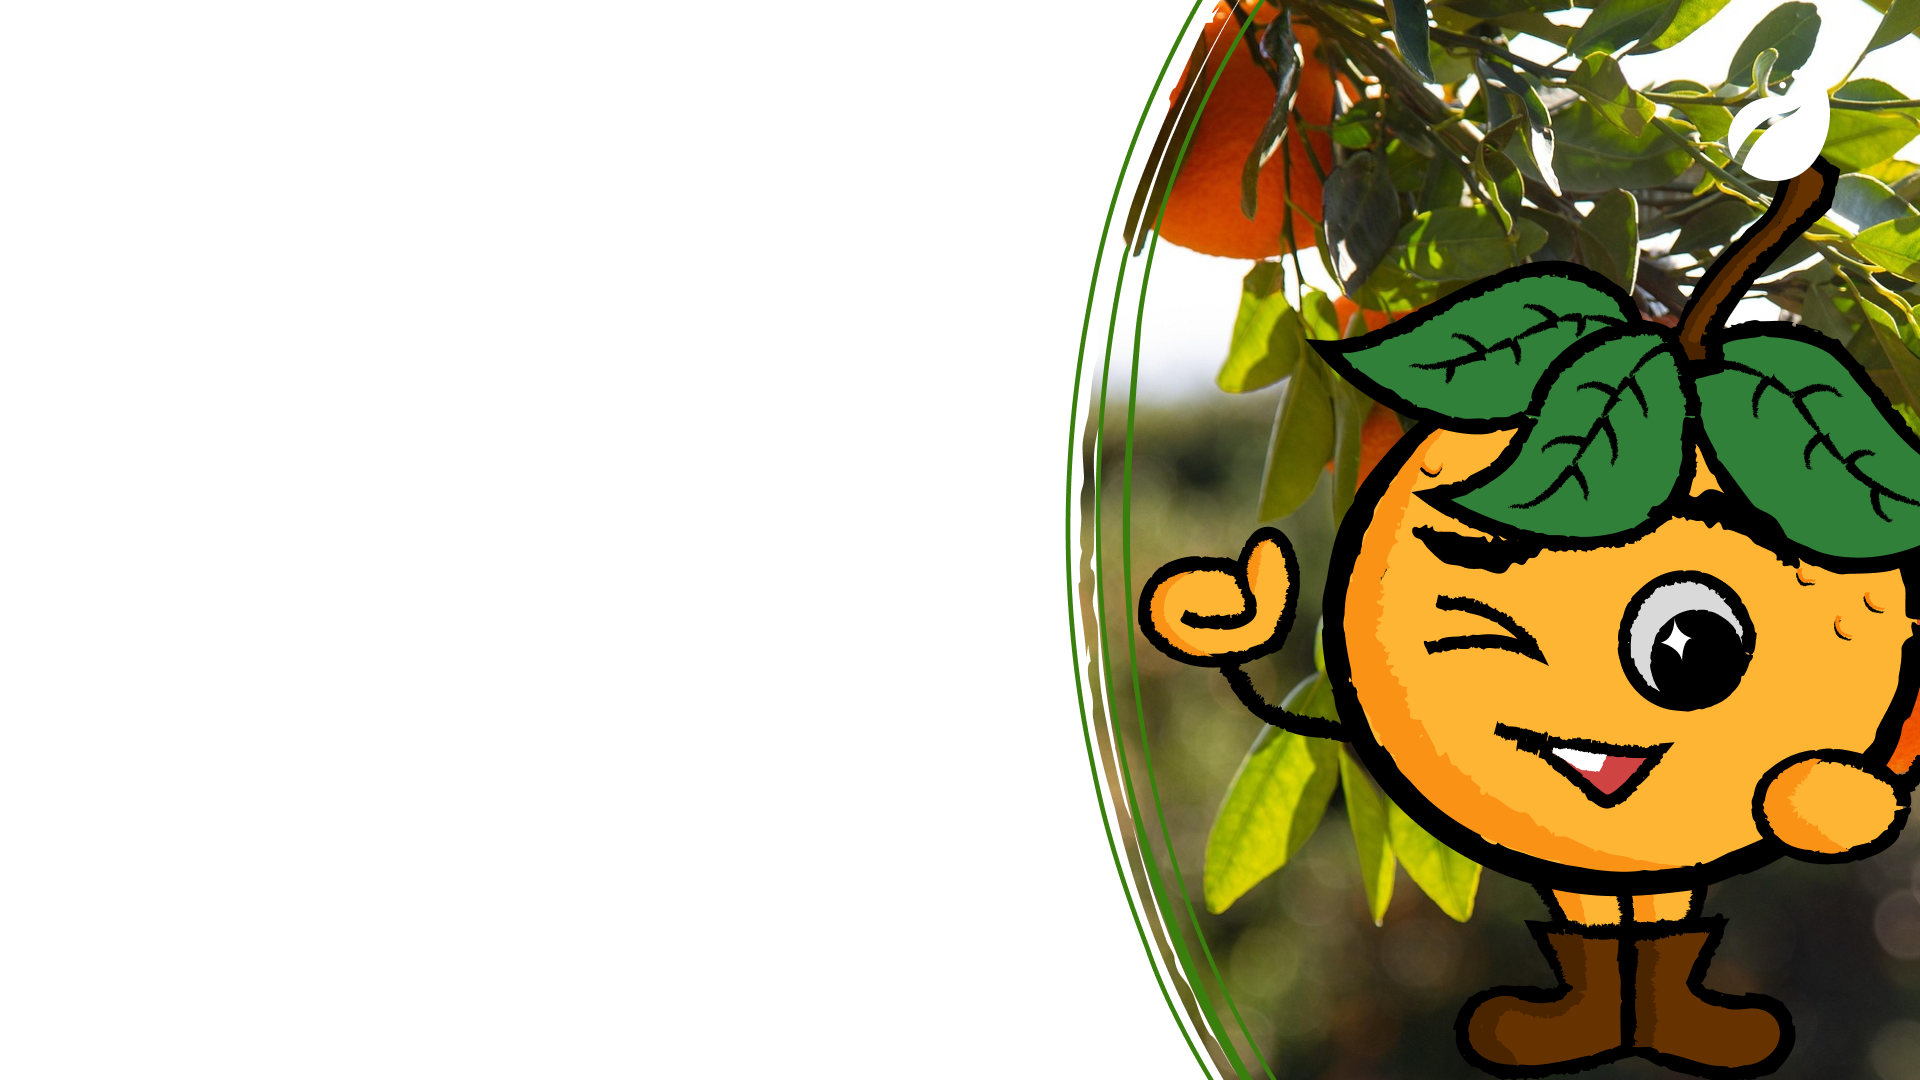
\includegraphics[width=\paperwidth,height=\paperheight]{imgs/Obrigado.png}%
}
\begin{frame}[b]{}
  \vspace{0.2cm}
  
  \hspace*{0.25\paperwidth}{\Large \textbf{Obrigado!}}
  
  \vfill
\end{frame}
}

\end{document}
